% This is "sig-alternate.tex" V2.1 April 2013
% This file should be compiled with V2.5 of "sig-alternate.cls" May 2012
%
% This example file demonstrates the use of the 'sig-alternate.cls'
% V2.5 LaTeX2e document class file. It is for those submitting
% articles to ACM Conference Proceedings WHO DO NOT WISH TO
% STRICTLY ADHERE TO THE SIGS (PUBS-BOARD-ENDORSED) STYLE.
% The 'sig-alternate.cls' file will produce a similar-looking,
% albeit, 'tighter' paper resulting in, invariably, fewer pages.
%
% ----------------------------------------------------------------------------------------------------------------
% This .tex file (and associated .cls V2.5) produces:
%       1) The Permission Statement
%       2) The Conference (location) Info information
%       3) The Copyright Line with ACM data
%       4) NO page numbers
%
% as against the acm_proc_article-sp.cls file which
% DOES NOT produce 1) thru' 3) above.
%
% Using 'sig-alternate.cls' you have control, however, from within
% the source .tex file, over both the CopyrightYear
% (defaulted to 200X) and the ACM Copyright Data
% (defaulted to X-XXXXX-XX-X/XX/XX).
% e.g.
% \CopyrightYear{2007} will cause 2007 to appear in the copyright line.
% \crdata{0-12345-67-8/90/12} will cause 0-12345-67-8/90/12 to appear in the copyright line.
%
% ---------------------------------------------------------------------------------------------------------------
% This .tex source is an example which *does* use
% the .bib file (from which the .bbl file % is produced).
% REMEMBER HOWEVER: After having produced the .bbl file,
% and prior to final submission, you *NEED* to 'insert'
% your .bbl file into your source .tex file so as to provide
% ONE 'self-contained' source file.
%
% ================= IF YOU HAVE QUESTIONS =======================
% Questions regarding the SIGS styles, SIGS policies and
% procedures, Conferences etc. should be sent to
% Adrienne Griscti (griscti@acm.org)
%
% Technical questions _only_ to
% Gerald Murray (murray@hq.acm.org)
% ===============================================================
%
% For tracking purposes - this is V2.0 - May 2012

\documentclass{sig-alternate-05-2015}
\usepackage[utf8]{inputenc}

\usepackage{listings}
\usepackage{color}

\begin{document}

% Copyright
\setcopyright{acmcopyright}
%\setcopyright{acmlicensed}
%\setcopyright{rightsretained}
%\setcopyright{usgov}
%\setcopyright{usgovmixed}
%\setcopyright{cagov}
%\setcopyright{cagovmixed}


% DOI
\doi{10.475/123_4}

% ISBN
\isbn{123-4567-24-567/08/06}

%Conference
\conferenceinfo{PLDI '13}{June 16--19, 2013, Seattle, WA, USA}

\acmPrice{\$15.00}

%
% --- Author Metadata here ---
\conferenceinfo{WOODSTOCK}{'97 El Paso, Texas USA}
%\CopyrightYear{2007} % Allows default copyright year (20XX) to be over-ridden - IF NEED BE.
%\crdata{0-12345-67-8/90/01}  % Allows default copyright data (0-89791-88-6/97/05) to be over-ridden - IF NEED BE.
% --- End of Author Metadata ---

\title{EnergyAware: Personal Energy Monitoring System}

%
% You need the command \numberofauthors to handle the 'placement
% and alignment' of the authors beneath the title.
%
% For aesthetic reasons, we recommend 'three authors at a time'
% i.e. three 'name/affiliation blocks' be placed beneath the title.
%
% NOTE: You are NOT restricted in how many 'rows' of
% "name/affiliations" may appear. We just ask that you restrict
% the number of 'columns' to three.
%
% Because of the available 'opening page real-estate'
% we ask you to refrain from putting more than six authors
% (two rows with three columns) beneath the article title.
% More than six makes the first-page appear very cluttered indeed.
%
% Use the \alignauthor commands to handle the names
% and affiliations for an 'aesthetic maximum' of six authors.
% Add names, affiliations, addresses for
% the seventh etc. author(s) as the argument for the
% \additionalauthors command.
% These 'additional authors' will be output/set for you
% without further effort on your part as the last section in
% the body of your article BEFORE References or any Appendices.

\numberofauthors{1} %  in this sample file, there are a *total*
% of EIGHT authors. SIX appear on the 'first-page' (for formatting
% reasons) and the remaining two appear in the \additionalauthors section.
%
\author{
% You can go ahead and credit any number of authors here,
% e.g. one 'row of three' or two rows (consisting of one row of three
% and a second row of one, two or three).
%
% The command \alignauthor (no curly braces needed) should
% precede each author name, affiliation/snail-mail address and
% e-mail address. Additionally, tag each line of
% affiliation/address with \affaddr, and tag the
% e-mail address with \email.
%
% 1st. author
\alignauthor
Nishad Gothoskar\\
       \affaddr{Carnegie Mellon University}\\
       \email{ngothosk@andrew.cmu.edu}
}
% There's nothing stopping you putting the seventh, eighth, etc.
% author on the opening page (as the 'third row') but we ask,
% for aesthetic reasons that you place these 'additional authors'
% in the \additional authors block, viz.
\additionalauthors{Additional authors: John Smith (The Th{\o}rv{\"a}ld Group,
email: {\texttt{jsmith@affiliation.org}}) and Julius P.~Kumquat
(The Kumquat Consortium, email: {\texttt{jpkumquat@consortium.net}}).}
\date{30 July 1999}
% Just remember to make sure that the TOTAL number of authors
% is the number that will appear on the first page PLUS the
% number that will appear in the \additionalauthors section.

\maketitle
\begin{abstract}
The "energy crisis" cannot be handled with just a single solution. Rather it demands a multifaceted approach. The part of the problem that we address in this paper is energy waste and unnecessary usage. The necessary step towards this goal is to give users insight into their usage breakdown and to see where the power they use is going. EnergyAware is a fully deployable system that allows us to provide exactly this for a user. This project is just as much social as it is technical. In a way, we are looking to change users' habits and usage patterns. The way we go about doing this is by providing them the necessary information to see what changes they should be making, along with the ability to execute these changes. EnergyAware is about allowing users to be aware of their energy usage habits.
\end{abstract}


%
% The code below should be generated by the tool at
% http://dl.acm.org/ccs.cfm
% Please copy and paste the code instead of the example below. 
%



%
% End generated code
%

%
%  Use this command to print the description
%
\printccsdesc

% We no longer use \terms command
%\terms{Theory}

\keywords{Belkin Wemo, Intel Edison, MongoDB, Twilio}

\section{Introduction}
Many times in the fields of Smart Buildings and Smart Homes, we disregard the essential concept of Energy Proportionality. In commercial buildings and residential homes, it may be true that there is a high inherent overhead and therefore proportionality cannot be achieved. But on a smaller scale, like apartments and single bedrooms that most young people live in, this proportionality is truly achievable, given that there is much less energy overhead. When we are not at home, our energy usage should be close to nothing and it should increase when we are present. But, the fact that our energy usage is not proportional should not be blamed on the users themselves. In fact many users would be readily willing to reduce their waste usage and adjust their overall usage. But power and energy usage measurement and statistics are not readily available or accessible to users, so they have no way of knowing how or in what ways they should change. In this paper we look to change this so users can be more aware of their energy consumption.

\subsection{Jevon's Paradox}
Jevon’s paradox says that when the efficiency of usage of a resource is increased there will be an increase in usage and demand and in effect there will be little to no change. While this may not be completely true when it comes to energy resources, it may be limiting our potential of energy savings. There is an aspect to Green Computing that can’t be solved by technological innovations alone. In some ways, significant improvement is dependent on changing user's usage and more importantly their demand habits. 

\subsection{Belkin Wemo}
Our measurement sensors are Belkin Wemo Insight Switches. These switches come with free software through an iOS and Android application. The application provides the ability to see minimal statistics about each plug and also control it remotely as shown in Figure 1. It is a quite thorough and useful application in theory, but practically it is hard to use and does not provide a solution to the problem we are attempting to solve. In this project we are not looking to remake or replace their existing application. Instead we are trying to extend and implement another aspect of energy management that the Belkin application was not meant for.

\begin{figure}
	\centering
	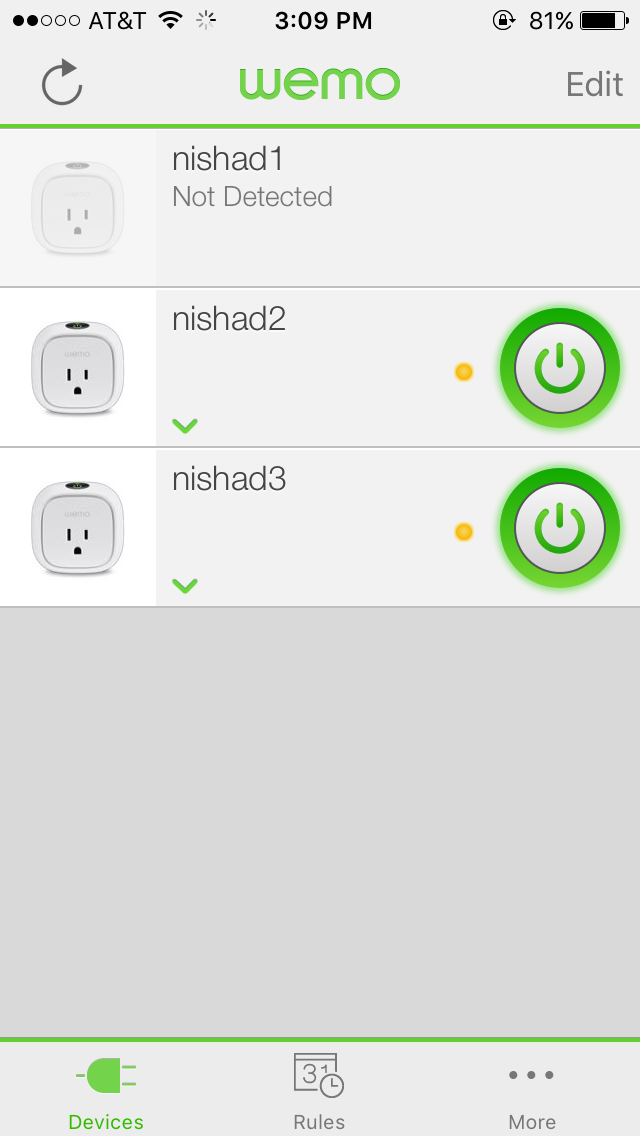
\includegraphics[scale=.15]{bel1} \ \ \ 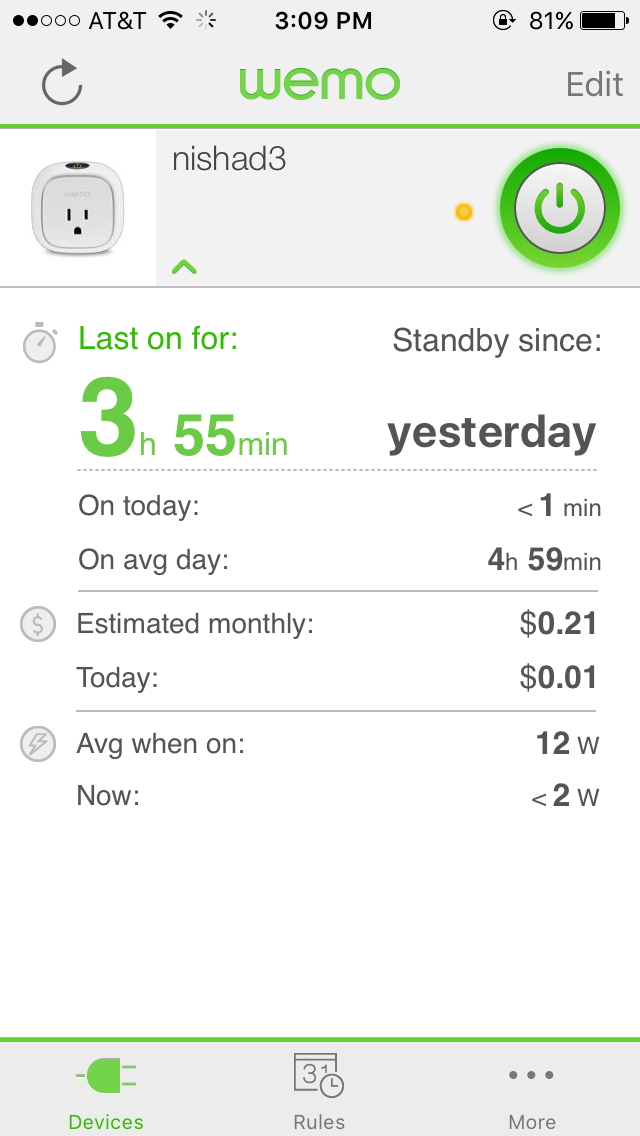
\includegraphics[scale=.15]{bel2}
	\caption{Screenshots from Belkin Wemo iOS App}
\end{figure}

\section{Hardware}
In the deployment of the EnergyAware system, we were conscious of the fact that it had to be easily deployable. Complex hardware setup would be unattractive to users and therefore the "market" for the system would be extremely limited. As mentioned above, the measurement is done by Belkin Wemo Insight Switches. These are WiFi connected devices which can be accessed by devices on the same WiFi network. The cost of these are around $\$50$ dollars each, which is on the more expensive side. However, we don't need these devices exactly since they have additional features that our system does not use which add to the cost. However sites like \texttt{openenergymonitor.org} have designs that can be made for much cheaper and would be sufficient for the EnergyAware system. Now, the second component is the center of our system, which runs all the main EnergyAware code. In our case, we ran it on an Intel Edison Breakout board, however it could be run on any system that will constantly be awake. Since it would be inefficient for someone to leave a desktop or laptop in there home on at all times, an Edison Board or any equivalent system like a Rasberry Pi would work well with little overhead.

\subsection{Power Ratings}
It is clear that we must ensure that our added hardware doesn't itself significantly increase energy consumption. Our system would be useless if we added a large energy overhead without significant savings. The Wemo Switch has a power usage of less than 1.5 Watts. Table 1 shows the ratings of the Intel Edison. It is clear that the power overhead of running EnergyAware is minimal and that adds to the inspiration of the system being something that can't hurt but only help improve habits and reduce wastage.

\begin{table}
	\centering
	\caption{Powering Intel Edison, Yocto 3.0}
	\begin{tabular}{|c|c|l|l|} \hline
		Activity&Power (mW)&Voltage&Current (mA)\\ \hline
		Booting Up& 944&4.97&190\\ \hline
		Using Wifi&803&5.02&160\\ \hline
		Idle&455&5.05&90\\ \hline
		Powered off&<51&5.12&<0.01\\
		\hline\end{tabular}
\end{table}


\section{Architecture}

The layout of the entire EnergyAware system stresses reliability and dependability. But, it also stresses usability given that this is a user-centric system and if the user does not enjoy/care to use it, it is almost meaningless. That is why, as you will see, there is quite a bit of modularity and data buffering even when many times it is not guaranteed to be used.

I like to think about the architecture as 3 main components: sensors, database, and manager. The manager sits between the sensors and database and initiates transactions of data between them. While there are other elements to the entire system, which will be discussed in a later section, they either extend or are a part of these main components of the EnergyAware system.

\subsection{Sensors}
On the sensor level, where you place the Wemo Switches is very important. First you want to ensure that every plug in the space is equipped with a sensor. These our outermost measurement points ensure that no power usage is unaccounted for and we have a direct way of measuring total energy consumption.

The next two metrics for deciding to place on a switch or not are power consumption level and actuation demand. Power consumption is critical because we want to make sure to place sensors on low power consumer but it is not necessary to have to do so on large power consumers. This is because it is easy to detect state changes in large devices just from looking at an outermost sensing point.  The second metric is actuation demand. If you want to be able to remotely control some appliance then you want to make sure to put it on a sensor and, to be most effective, group together devices that you want to be able to turn off together, say the group of devices that you want to be off when you leave the house.

So, we categorize devices with Level 1 being the outermost socket sensors. We have this level so it is easy to compute total power usage by summing over Level 1 readings. Level 2 begins the devices we want to measure and be able to actuate when we are not home. Level 3 are all other devices. This organization comes in handy when it comes to complex implementations.

The other categorization is devices that we want to be off when we are  not at home. So we also label devices with a tag that identifies if they are occupancy dependent or not.

\[
\begin{cases}
Socket 1 - 1
\begin{cases}
Light1 - 2\\
Laptop - 3\\
Monitor1 - 2\\
Monitor2 - 2\\
\end{cases}\\
Socket 2 - 1
\begin{cases}
Phone-3\\
Light2-2
\end{cases}\\
\end{cases}
\]

We have here an example plug structure.

\subsection{Database}
Our databases are an essential part of the system architecture as the allow for data and information flow. Most of the information is passed as JSON objects as that is what works well with MongoDB, the database we chose for this implementation. We have a few databases that each serve a separate but essential purpose in the entire system's functionality.

The first two databases are the \texttt{wemo.names} and \texttt{wemo.ips} databases. The names database designates which switches on the network to be considered in our system. Because the Wemo switches are WiFi enabled, anyone on the network can see them. Many times campus residents share a Wifi network and our system would not want to include all the sensors on the network, because they might not all be owned by the user, so we have them specify which sensors to include. The second database asks for the IP addresses of all network connected devices which a user possesses. We will discuss the purpose of this later in the paper.

The next databases is \texttt{wemo.todo}. This is essentially our instruction stack. Instructions are popped off the stack and execute by the central system. This database is extremely restricted because it actually poses security and privacy concerns due to the ability of changing states of a users devices.

The final two databases are about information storage. These are \texttt{wemo.reading} and \texttt{wemo.state}. Our reading database is what we write all the power reading from each of the sensors to. Our state databases is where we write state change events to.

The databases feed other components on top of the system that look to it for information. While the manager also plays a part in this, both need to ensure that the data that is being passed backwards is presentable, whether that be by smoothing, analytics, or other tools.

\subsection{Manager}

The manager is the central piece to the entire system. It is what connects all the components and manages the registered devices. Since it is so central, we have made it as fault tolerant as possible. However in the case that it does break, we don't want to have the system down for long periods and without anyone knowing, so we have a fault alert system that will alert users before the script shuts down.

The manager runs on the Intel Edison boards and requires constant power. But fortunately, in the case of power outages or faultiness, the script will automatically start itself again and because of the way it is written, it will miss/lose little to no information at all.

\section{Core Implementation}

Our implementation was primarily in Python and various REST interfaces. I chose Python for this project because of my experience with it and also for how easily it works well with many of the technologies (software and hardware) that we are working with.

\subsection{Sensors}

The Sensor setup is the one part that we weren't able to integrate into our system. The setup process is long and tedious and encounters many issues. We are forced to use the Wemo application for iOS and Android to setup the sensors with a name and Wifi connection.

However after that point, but before you power on the Intel Edison board, you must register the devices through the entirely web interface and proceed with the setup of your "personalized" system. At that point you will plug in the Intel Edison board and the script will import all the data you entered to initialize the system properly.

\subsection{Databases}

We have discussed how each of the other components uses and interacts with the databases, but have never discussed the format in which it holds data and the schemas that it adheres to. Our databases are listed below:
\begin{center}
	\texttt{wemo.reading}\\
	\texttt{wemo.state}\\
	\texttt{wemo.todo}\\
	\texttt{wemo.err}\\
	\texttt{wemo.names}\\
	\texttt{wemo.ips}
\end{center}

The structure of the databases adheres to the following standards, but ignores what is not pertinent to the individual databases purpose:
\begin{flalign*}
&\texttt{reading: $\{$"time":-,"name":-,"nick":-,"data":- $\}$}\\
&\texttt{state: $\{$"time":-,"name":-,"change":{on/off}$\}$}\\
&\texttt{todo: $\{$"data":-$\}$}\\
&\texttt{err: $\{$"time":-,"id":-$\}$}\\
&\texttt{names: $\{$"name":-,"nick":-,"level":- $\}$}\\
&\texttt{ips: $\{$"ip":-$\}$}\\
\end{flalign*}

\subsubsection{REST Interface}

At first we tried to build our system off the existing HTTP interface that exists for MongoDB. This worked well until we realized that it was limiting our JSON return results to at most 1000 rows. Given that we read our sensor data at a high granularity, this data base fills up past 1000 rows quite quickly.

Many times this does not become an issue, especially if we are interfacing with that database with Python. But when we are using Javascript, as we do in our front end, we need to have a way to serve all the data as a JSON. That is why we have a REST interface that runs on our DigitalOcean server, that serves the requested JSONs and preprocesses the data so it is readable and easier for the front end developer to work with.

\subsection{Manager}

The manager is our \texttt{main.py} that is constantly running on the Intel Edison board. Since this a main component of the system, it stresses efficiency and fault tolerance. To start the manager and therefore the EnergyAware system, all you must do is supply power to the system. It will automatically startup the codebase and send a message to verify it has started up properly since the Intel Edison has no GUI to display errors or issues.

\subsubsection{Initialization}

The first thing it does is gather the necessary data from the various databases. From this it constructs a dictionary that maps \texttt{Sensor Name} to \texttt{(Sensor Level, Nickname)}. This Sensor Level concept is discussed in the architecture section but essentially it represents its place in the sensor hierarchy. Many times the Sensor name is complex or random, so the Nickname is a more user friendly way to reference the sensor. The nickname can be something like "Laptop", "Light1", etc. 

Now, since many time when taking input from the user we would like to be able to handle them referring to sensors by their nickname, we also have a dictionary \texttt{nicknames}. This simply maps a nickname to the sensor name which helps other later components later.

\subsubsection{ouimeaux}
The ouimeaux libraries allow Python to interface with the Wemo Insight sensors. The ouimeaux module is Open Source so we are allowed to use it in our system.

Using this system, the next step in our process is to do a scan on the network for \textit{any} Wemo device. That is why it is essential, above, to keep track of all Wemo switches that the user registers as their own. So after the scan we only keep the registered switches as create our \texttt{switchmap} that maps switch names to the actual switch object. This switch object is the one we interact with for control and information on the switch.

With the ouimeaux library we request various pieces of information from the switches. In our implementation we query for 3 pieces of data: todaykwh, currentpwr,todayontime. These pieces of data give as an instantaneous sense of usage with power, a cumulative usage estimate with power, and also a sense of the "on time" of the devices we use.

\subsubsection{Data Accumulation Loop}
This loop will execute every \textit{x} seconds. This x is given as a command line argument when starting the main script. In each iteration of the loop we do the following:
\begin{enumerate}
	\item Get data from sensors
	\item Detect sensor level state changes
	\begin{enumerate}
		\item Check if 0 to nonzero (on)
		\item Check if nonzero to 0 (off)
	\end{enumerate}
	\item Increment total if level 1 sensor
	\item Write all data to database
\end{enumerate}

We keep track of the total data (across all assigned Level 1 Sensors) because that is probably what a user would like to see. The system is designed to get users the energy information that is usually inaccessible. They are probably most interested in their overall usage patterns.

\subsubsection{Occupancy sensing}

While the occupancy is part of the loop pattern above, we give it another section here because of its significance to the system as a whole. Our occupancy sensing isn't as rigorous or thorough as other occupancy sensing projects. A user will have a registered set of devices and IPs and we monitor the presence of these devices on the network to "measure" occupancy. This is done by simply calling \texttt{subprocess.call(['ping', '-c', '3', ip])}.

A challenge of the occupancy sensing, which was only discovered recently, is that in iPhone's, the network hardware will go into sleep state when the phone goes to a sleep state. This was originally throwing off all our occupancy readings to be when the device is in use. However we now use a clever method (this was not discovered by me \cite{tcp}). The \texttt{port 62078} on the iPhone is known as the \texttt{iphone-sync} port and is used to connect to iTunes and sync. We can issue a \texttt{tcping IP 62078} and will receive a response even when the phone is in a sleep state.

I am also working on incorporating bluetooth scanning for a set of devices to do the same. We came upon this idea by realizing that a later component, Physical Web sensors, is also dependent on bluetooth so it is likely that a user of this system will have their bluetooth on as well. The bluetooth sensing works if you run the system from your desktop but is not yet implemented on the Intel Edison. However, this bluetooth component is not essential to the performance of the EnergyAware system.

The occupancy sensing is not done at the same granularity as the sensor reading. This is under the assumption that the user of the system will not be entering and exiting within a matter of seconds and even if they did, accounting for it would have little effect on how our system functions. This design decision also is conscious of not having to send unnecessarily many pings to your devices.

\subsubsection{Fault Tolerance}

Given that we are running the manager on an Intel Edison or equivalent board, we are not giving feedback to the user. Therefore, to give them an update the the system has started, we send a text message alerting "System Start". We also send a message alerting "System Stop" if the script ever stops running. This way, they can assess and report an error to be resolved, and there is never a situation where the user believe the EnergyAware system is running when in fact it is not. Finally, as discussed in the first paragraph, we need to give alerts when we hit errors, however not just to the users, but to us as developers as well. So before exit, the script will also write to an error database with the MAC address of the machine its running on. This allows us as the developers to diagnose and fix issues.

Since many of the calls and data reads are dependent other networked hardware, there is a chance that something malfunctions and we can't get a reading. This is not in our codebase, rather in the Python libraries and actual Wemo devices, so we can't fix the issue but instead must learn to handle these errors. The first way we do this is by assigning timeouts to all network dependent functions. This ensures that we never get stuck waiting when a sensor has dropped off line and can continue with the next iteration of the loop. Also, given that we don't know the errors or steps that the ouimeaux library takes to read data from the sensors, we also have wrap all their function in \texttt{try...except...} handlers to prevent the script from crashing.



\subsection{Instruction Stack}

The manager as described above is limited to outward interaction. It gets data from the sensors, it sends data to databases, and it sends messages to the user. But at its current state, there is no way for anything outside the codebase to interact with the system. This why we have the Instruction Stack and why its an integral part of the interaction with EnergyAware

The instruction stack is implemented itself as a database. The manager loop will every so often (not at the same rate as sensor readings) will read and delete all the data from the database. Then according to some protocol it will execute these instructions. We will talk about the various functions of the instruction stack later in this section. Below are described the various methods of interaction, however keep in mind that this can be generalized to any method of interaction given how generally our instruction stack structure is designed. Being a set of string representing instructions, any device that can post to a database is capable of being programmed to interact with the Energy Aware system.

Our system is designed to be able to accept turn on and turn off instructions, as well as queries to check the state of a device.

\subsubsection{Twilio}

One of the various methods of interaction in the EnergyAware system is through text messaging. To allow us to send and receive messages, we use the Twilio service. Twilio gives us a dedicated phone number that we can interact with using HTTP. On our Digital Ocean droplet (which is discussed in a later section), we constantly run a HTTP server using Python that takes the text received from the message, parses it properly, and inserts it into the Instruction Stack database.

The first text message based interaction is changing the state of devices. The instruction for this is of the form:
\begin{equation*}
\texttt{\{turn,switch...\} \{name,nickname\} \{on,off\}} 
\end{equation*}
The next message based interaction is getting the state of the devices. And to do that, we pass:
\begin{equation*}
	\texttt{is \{name,nickname\} \{on,off\}} 
\end{equation*}

Now we want to make sure, from a user interaction/usability perspective, that we are selective in what we automatically send the user. We want to give the user alerts and messages, but we don't want to bombard them with unnecessary messages because this reduces the attractiveness of using EnergyAware. So we allow them to choose preferences for how they will receive messages.

We can also use the Twilio system for sending two other alerts about the data that we collect. As we will later discuss in the front end, we allow the user to set daily energy usage and time usage quotas. When users reach certain percentages in their quotas we can send them text message alerts that they have used that percentage.

Also, we can alert users when they are not at home that they have left devices on. We do this for devices that are marked 

\subsubsection{Security}

While security is an important part of the entire EnergyAware system as a whole, it is particularly important here. Security of the instruction stack is essential, because without it, we could have tampering with devices on and off state or overloading the Instruction Stack. We have various methods of securing, as discussed below.

The first method is simply just with username and password on the database. All elements that need to access the database to read or write know the username and password and none of these elements are forward facing, meaning they are either embedded in a script or hidden by a \texttt{.htaccess} requirement.

Now the next layer of protection involves the \texttt{iptables} that restrict the IP addresses that the Mongo server accepts connection from. This reduces the damage that an attacker trying to bombard the database could do.

Finally, a security measure that is natural implemented in Twilio, not done by us, is restricting the phone numbers that we can send messages to. But the measure that we have added is restricting the phone number that can message our Twilio number by filtering out messages that come from unregistered numbers.

\subsubsection{Integration with Manger}
The code for how this operates with the manager is below and is quite straightforward:

\DeclareFixedFont{\ttb}{T1}{txtt}{bx}{n}{10} % for bold
\DeclareFixedFont{\ttm}{T1}{txtt}{m}{n}{10}  % for normal

% Custom colors

\definecolor{deepblue}{rgb}{0,0,0.5}
\definecolor{deepred}{rgb}{0.6,0,0}
\definecolor{deepgreen}{rgb}{0,0.5,0}


% Python style for highlighting
\newcommand\pythonstyle{\lstset{
		language=Python,
		basicstyle=\ttm,
		otherkeywords={self},             % Add keywords here
		keywordstyle=\ttb\color{deepblue},
		emph={MyClass,__init__},          % Custom highlighting
		emphstyle=\ttb\color{deepred},    % Custom highlighting style
		stringstyle=\color{deepgreen},
		frame=tb,                         % Any extra options here
		showstringspaces=false            % 
	}}
	
	
	% Python environment
	\lstnewenvironment{python}[1][]
	{
		\pythonstyle
		\lstset{#1}
	}
	{}
	
	% Python for external files
	\newcommand\pythonexternal[2][]{{
			\pythonstyle
			\lstinputlisting[#1]{#2}}}
	
	% Python for inline
	\newcommand\pythoninline[1]{{\pythonstyle\lstinline!#1!}}
\begin{python}
... Outer Loop ...
s=db.find()
s=[i["data"] for i in s]
for instruct in s:
	i=[ins.lower() for ins in instruct]
	execute(i)
db3.delete_many({})
\end{python}

\section{Further Implementation}

So everything discussed previously consists of the barebone essentials of the EnergyAware system. But any useful and complete system is built to be expanded and extended upon. We kept this in my mind while designing the system as you will see in the following sections.

\subsection{Updates}

We have a system in place so that even if the EnergyAware is already deployed, we can remotely change the code when we receive reports of errors. Already described in an earlier section is the \texttt{wemo.err} database that we can monitor to see errors and on which deployments of the system they occurred on.

With that we can make changes where necessary. The main.py script will only execute after sending a request with the current version number to:
\begin{equation*}
	\texttt{http://www.nishadg.com:8082} 
\end{equation*}

And if the version is not the current one, it will get the next version main.py at:
\begin{equation*}
	\texttt{http://www.nishadg.com/update} 
\end{equation*}

There is a security flaw here that I am working on researching how to be able to serve an update without allowing a user to look at what it consists of.

\subsection{API}

The EnergyAware system was designed so that 3rd parties could write "applications" on top of the underlying system. The term applications does not exactly fit here, rather you would be able to add your own routine that will execute along side the existing codebase. We here provide a Documentation of the API for this programmable additional routine.

EnergyAware will pass you the following data structures as described earlier in this paper:

\begin{enumerate}
	\item switchpair: sensor name to sensor object
	\item nicknames
	\item devicemap: sensor information
\end{enumerate}

Now the EnergyAware system also requires some restrictions on the "applications":
\begin{enumerate}
	\item integer exectime (expected execution time)
	\item function appname (function to execute)
	\begin{enumerate}
		\item Must take 3 parameters as described above
		\item Must execute in exectime seconds
		\item Must not change passed argument
	\end{enumerate}
\end{enumerate}

All this must be packaged in a file named appname.py. And all the apps must be stored in directory (at the same level as the main.py) named \texttt{apps}. Sometimes you will need to include an empty \texttt{$\_\_$init$\_\_$.py} file in the app and upper level directory

Now in our main script, we will first import all these "apps" and store the corresponding functions and exectime's in a list. We have a user specified loop interval, but we want to ensure that the sum of the exectime's is not more than the interval, since this could lead to unexpected side effects. So, we sort all the functions by their exectimes and execute only up until the point where the sum of the exectime's is less than the user defined interval. This is all under the assumption that if a user wants to use more applications, they will choose a larger interval.

Now, to enforce the exectimes and ensure that an app doesn't just maliciously take up time, we use the same timeout library as we used on our own code and apply that to user code.

The protocol described is implemented as such:
\begin{python}
f=os.listdir("apps")
f=[t for t in f if ".py" in t]
apps=[]
for app in f:
	name=app[:-3]
	modname="apps."+name
	t=__import__(modname,fromlist=['']) 
	apps.append((t.appname,t.exectime))
\end{python}

\subsection{Data Analysis}

The ML portion of the project was an element that we were not able to complete to its entirety. We have worked out analyzing the data and learning from it, but we have not implemented feedback from it. So, the results of learning are not fed backwards to the system so that it can adapt. So in this section we will discuss the analysis we did of the data.

The first thing we did is look just at occupancy data. With occupancy data you can look for routines. Our occupancy data is represented by a graph that takes on values of 0 and 1 over time. Alone this data is not interesting, but averaging all these together gives you a smoother average occupancy over time. We can take advantage of the patterns we see here. With this, we have a probabilistic model of whether a user is at home.

The next analysis was on a device level. In our \texttt{wemo.state} database we have marked transitions of devices and their times. Now from that we can look at routines of device usage. For example, lights turning on and off at certain times.

\subsection{Physical Web Beacons}

The next element was inspired by what I will be working on this summer. The concepts of Smart Home, Smart Meter, etc. are extensions of what is commonly referred to as the Internet of Things. The Physical Web beacons are Bluetooth beacons that transmit URLs. The concept is quite simple, but that is for a good reason, because it is a concept that can generalize to everyday objects.

For our project we wanted to extend this concept to our outlets and power usage in our home. The inspiration for my entire project was let people have access to this new set of data that was previously entirely unaccessible. The Physical Web beacons are trying to create a new level of interaction, and in this application, we want to allow users to be able to "interact" with their home power supplies in a way that was previously not possible.

Currently the beacons are larger and not integrated into the power meter, as shown in Figure 3. But we hope that later, this kind of technology will be built into the sensors, as it is quite low power and efficient.

\begin{figure}
	\centering
	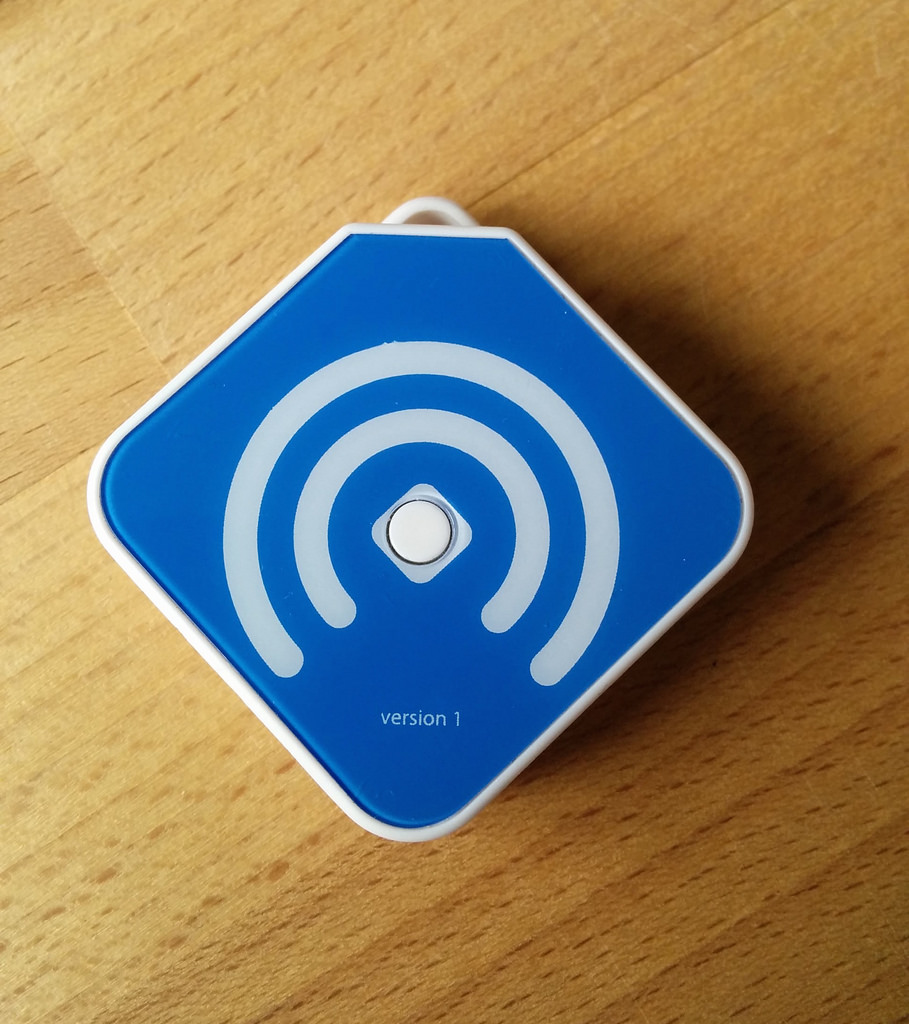
\includegraphics[scale=.1]{phys}
	\caption{Physical Web Beacon\cite{physweb}}
\end{figure}

What the beacons are programmed to do is transmit a URL that represents its corresponding power meter. And this URL essentially represents a "homepage" of that power meter. It gives us readings of total power usage, a graph of its power usage, and the ability to switch a sensor on/off. We wanted to keep it simple since it was a user friendly "insight" into the outlet. A sample of what this energy dashboard looks like is shown in Figure 4.

\begin{figure}
	\centering
	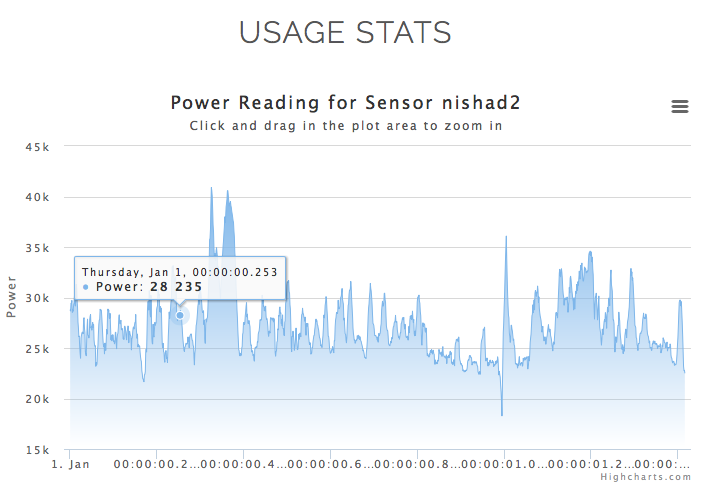
\includegraphics[scale=.34]{phys2}
	\caption{Sensor Dashboard}
\end{figure}

\subsubsection{Security (Extended)}
It was at this point that we realized that since we are transmitting a signal about the power meter that anyone could see, we needed to add another higher and complete level of security. So, we turned the entire system into an account based system where you needed to register and login before being able to access any data.

\subsection{Front End}

As just described above, at \texttt{www.nishadg.com/wemo}, you have must first login and be authenticated. You then have access to the Energy Dashboard.

You will first see a list of all the sensors that we have data on and short profiles about them. This is supposed to give you a way to compare these sensors, when compared to the individual view that the Physical Web beacons give you. They also have links to be able to see the individual, in-depth dashboards.

The next parts are to be able to see an overall view of your energy and power usage habits and characteristics. These include the total power usage readings graph. This gives you a sense of how your power usage varies over the day, over the month, etc. The Highcharts API has a useful graph mode that lets you zoom in and out to get a better view

In our midterm presentation, we made it a point that we wanted to try to change our users behavior. And, two methods we saw of doing this was by using Tradeoffs, Money, and Competition. Below we illustrate our various means of doing this.

In our abstract we discussed this concept of energy proportionality. If we graph the power consumption of a user with respect to occupancy (though occupancy in our sense is a discrete measurement), we can look at this line and have a sense of energy proportionality. While the slope of this line does't exactly tell us the energy proportionality, since the y-intercept plays a part, it does give a sense of how much changes when a user is home when compared to a user not being home. So our measure of energy proportionality is as follows:
\begin{equation*}
\begin{split}
AHU = \frac{(M_{1}+M_{2}...+M_{10})}{10}\\
ANHU = \frac{(M_{11}+M_{12}...+M_{20})}{10}\\
Score = (AHU-ANHU)/AHU
\end{split}
\end{equation*}
Where AHU is the average home usage, ANHU is the average not home usage and your score correlates to your percent decrease when you're not at home. The M values are random samples of home and not home power readings. We thought to just average all that data, but realized that if this system runs for longer periods of time, that is quite an expensive operation and is not entirely necessary.

The other metric we present is cost. Since we can't be too fine grained about a cost measurement since we do not have statistics about it, we just place the traditional $\$0.12$ per kWh and compute that on total usage. We also do that computation daily to give a sense of how much you aggregate in costs of electricity per day.

Now, we can add the competitive element to this data by presenting the data to the user properly. In Figure 4, we have created some fake data for users since our system has not had many users. You can see the distribution of scores and the shaded area represents all the users that are doing better than yourself.

\begin{figure}
	\centering
	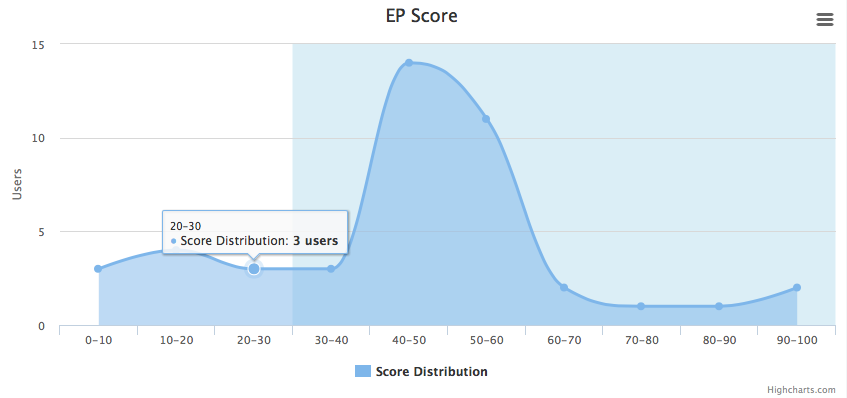
\includegraphics[scale=.3]{dist}
	\caption{Energy Proportionality Score Distribution}
\end{figure}

\section{User Study}
We hope to deploy this system to many users. But obviously before we can do that we need to test the system on real users in a control system. While our user study is not entirely rigorous or thorough, it did give us a sense of what changes needed to be made and what issues the system had. But at the same time, it showed us that our system did have an effect. What is discussed in this paper is not entirely what was deployed to the user, because after the feedback, we implemented the necessary changes.

I deployed the system to a user who had a moderately technical background. All I gave him was a set of 3 sensors and an instruction sheet on how to setup the system. He used the system for about a week and his comment on the system was:

"It was fascinating to have a system in which you can power on and off your devices and see your usage of power. Although there are system like it in the market, I really like the fact that you can control it by a text message rather than having to download an app. Also it is mind opening to be able to see the carbon footprint you are leaving in this ever evolving world. There are still some issues, like connecting to Wifi and some bugs in the web interface."

From my own observations, I could see that he was able to setup the system quite quickly, correctly connecting the sensors and powering on the Intel Edison. His use of the system was proper, in that he was conscious about reducing his power after he realized he could see a drop in the usage and power readings graph. He also mentioned that it did not hinder or negatively effect him in any way. While this is not really an achievement of any sort, it is an important factor to consider. If the costs of a system are too high, users have no incentive to use it. According to our users account the costs are close to nothing, so any assistance the system provide are "profits".

\section{Challenges}
The first main challenge with this project was the architecture. It was modified many times before we settled on the current model. It was important because we had to insure that the data we needed was in the right place at the right time. What we mean by that is, all the preprocessing work must be handled by the backend so that when a user accesses the front end web application, all the data is ready to be loaded instantly and there is no latency.

The next challenge was how to store data so that it would be a formatted properly for all dependent elements to access. A pertinent question here was do we store all data recorded in one iteration of the loop together a one entry or a separate entry for each sensor so we can easily run filters and move data around.

The last challenge that was clear in this paper was the Machine Learning aspect. While all the methods are setup and written to do so, it is hard to integrate the data back into the system. Most machine learning problem involve learning and optimizing an algorithm, but in our case, we are trying to optimize a person's behavior. I believe that this component will be in future work and will be easier with more users and more data to look at.

\section{Future Work}
The future work on this system is in two main directions. The first is to incorporate the Data Analytics and provide feedback to the user and to the system from it. Where I see it being used most, is to learn the routines of usage on devices and predict when a user has made a "mistake", meaning they left a light on while they are away. This will take the effectiveness to another level because not only will it help users turn off devices that they know need to be off, but it will predict when devices should be off without the user not even defining it. In terms of the system, this involves learning what Level 2 and Level 3 sensors are and how to find Level 3 sensors that should be Level 2.

The other directions is users being able to "download" applications from an App Store style system that can let them have apps for certain sets of devices. For example, a Washing Machine Cost optimizer that looks at energy "deals" to help you improve your usage. Or, a system that turns on your lights at a certain time to wake you up and turns off devices at a certain time to make you go to sleep. While many of these apps already exists, they can't be used on a centralized system and be coordinated. That's what EnergyAware can provide for these applications.
\section{Conclusions}
With this system we sought to address a major problem in how we manage our energy usage. We have learned to be conscious of wasting energy, but it is hard to truly know \textit{where} energy is wasted. So in fact, part of the problem is the inaccessibility of information.

EnergyAware provides a solution to this problem. Its main goal is to provide insight and visibility into where our energy is going. We kept in mind dependability and scalability in designing the system so that it can be improved and extended.

The concept of the Internet of Things is about utilizing the interconnectedness of devices and sensors in an intelligent fashion. In our case, it is about aggregating data and analysing, parsing, and presenting it in useful manner. While there are many Building OS style projects out there, EnergyAware is our take on a personal level energy management system.
%\end{document}  % This is where a 'short' article might terminate

\begin{thebibliography}{9}
	\bibitem{tcp} 
	Apple. 
	\textit{TCP Port 62078 on my iPad is open}\\ 
	\texttt{https://discussions.apple.com/}
	
	\bibitem{physweb} 
	Google.
	\textit{Physical Web}\\ 
	\texttt{https://google.github.io/physical-web/}
\end{thebibliography}
%ACKNOWLEDGMENTS are optional
\end{document}
